\begin{figure}[h]
\centering
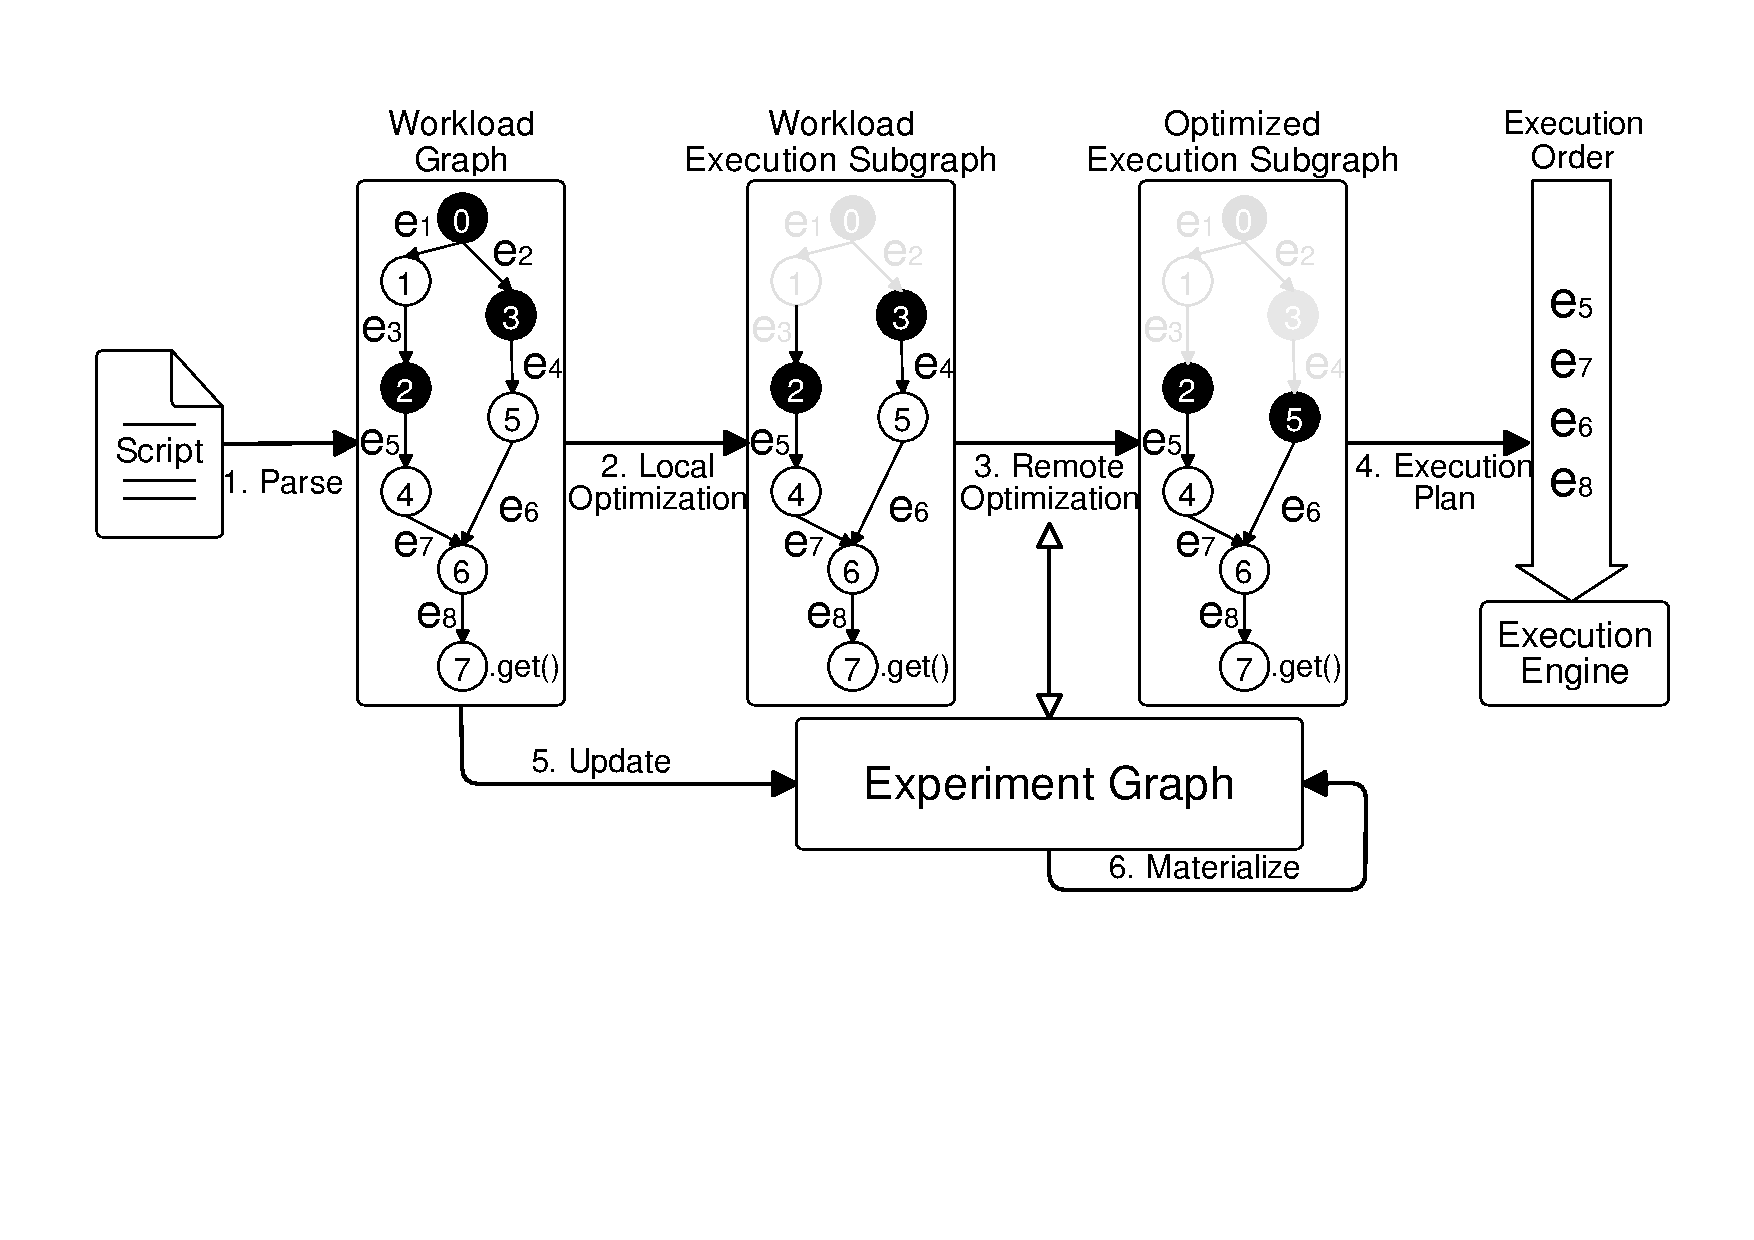
\includegraphics[width=0.9\columnwidth]{../images/system-workflow}
\caption{Overview of the collaborative workload optimizer system}
\label{system-workflow}
\end{figure}
\section{Collaborative ML Workload Optimizations} \label{sec-ml-workloads}
In this section, we provide an overview of our collaborative ML workload optimization system.
Figure \ref{system-workflow} shows the high-level architecture of our system.
Similar to collaborative environments, our system also comprises of a client and server component.
The client is responsible for parsing the user workload into a DAG (Step 1) and pruning the workload DAG (Step 2).
The server receives the workload DAG and utilizes our reuse algorithm to optimize the DAG (Step 3) and sends it back to the client.
Finally, the client executes the optimized DAG (Step 4) and prompts the server to update the Experiment Graph and store the artifacts of the executed workload DAG (Step 5).
This architecture enables us to integrate our system into the existing collaborative environments without requiring any changes to their workflow.
Similar to collaborative environments, the client and server can run within a single cloud environment where each client is an isolated container.
In the rest of this section, we describe the process of parsing, pruning, generating workload DAGs, and executing the workloads.
Then, we describe the process of constructing the Experiment Graph and how we utilize the Experiment Graph in our materialization and reuse algorithms. 
Finally, we show the integration process and the impact of our system on our motivating example (described in Section \ref{sec-background}).
\subsection{Client Components}
\textbf{ML Script and Parser.}
Instead of designing a new DSL, we extend the existing Pandas and scikit-learn \cite{sklearn_api} python packages that are common choices for data analysis and machine learning workloads.
Upon invocation of the program, the parser reads the script and transforms it into a DAG.
Listing \ref{listing-simple-workload} shows an example of a workload script.
The goal of the workload is to process a dataset of item descriptions, prices, and whether or not the items were purchased and train a classification model to predict whether new items will be purchased or not.
With only a slight modification of the import commands, we can load our parser modules.
As a result, we can support both long-running python scripts and interactive Jupyter notebooks.
\begin{lstlisting}[language=Python, caption=Example script,captionpos=b,label = {listing-simple-workload}]
import custom_pandas as pd

from custom_sklearn import svm
from custom_sklearn.feature_selection import SelectKBest
from custom_sklearn.feature_extraction.text import CountVectorizer

train = pd.read_csv('path-to-datasets/train.csv') 
print train.columns # [ad_desc,ts,u_id,price,y]
ad_desc = train['ad_desc']
vectorizer = CountVectorizer()
cnt_vect = vectorizer.fit_transform(ad_desc)
selector =  SelectKBest(k=2)
t_subset = train[['ts','u_id','price']]
y =  train['y']
top_feats = selector.fit_transform(
                                  t_subset,  
                                  y )
top_features # print the content of the data frame		     
X = pd.concat([count_vectorized,top_features], axis = 1)
model = svm.SVC().fit(X, train['y'])
print model # terminal vertex
\end{lstlisting}

\textbf{Workload DAG.}
In our DAG representation, vertices are the artifacts, i.e., raw or preprocessed data (represented by data frame objects) and machine learning models resulting from feature engineering and model training operations and edges are the operations in the workload.
Each workload DAG has one or more vertices representing the raw datasets.
We refer to such vertices as sources.
A workload DAG also contains one or more terminal vertices.
Terminal vertices represent the output of the workload.
For example, a terminal vertex is a trained ML model, a preprocessed dataset, or aggregated data for visualization.
Requesting the result of a terminal vertex triggers the optimization and execution of the workload DAG.
Figure \ref{fig-workload-dag} shows the workload DAG constructed from the code in Listing \ref{listing-simple-workload}.
In the Figure, the highlighted vertex represents a terminal vertex, which is the result of the print statement on Line 21 in Listing \ref{listing-simple-workload}.

\textbf{Local Pruner.}
Once the user requests the result of a terminal vertex, the client prunes the DAG before sending it to the server.
The task of the pruner is to identify all the unnecessary edges.
There are two groups of unnecessary edges: edges that are not in the path from source to terminal and edges with their endpoint vertex already computed.
The latter is very common in interactive workloads since every cell invocation in Jupyter notebooks computes some of the vertices.
As a result, in the future cell invocations, previously executed operations can be skipped.
Note that the pruner does not remove the unnecessary edges from the DAG and only marks them as inactive.
For example, in Figure \ref{fig-workload-dag}, if \textit{t\_subset} is previously computed, the local pruner marks the edge between \textit{train} and \textit{t\_subset} as inactive.
After the pruning, the client sends the DAG to the server.
To minimize the transfer cost, the client does not send the content of the computed artifact to the server.
\begin{figure}[h]
\centering
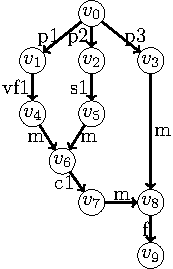
\includegraphics[width=\linewidth]{../images/tikz-standalone/example-graph}
\caption{Workload DAG constructed from the Listing \ref{listing-simple-workload}. The highlighted node shows a terminal vertex.}
\label{fig-workload-dag}
\end{figure}
\vspace{-2mm}

\textbf{Executor.}
After the server optimizes a workload DAG, the executor receives the optimized DAG to execute the operations and returns the result to the user.
The executor runs the operations in the optimized DAG in their topological order and returns the result to the user.
To avoid redundant computation, the executor ignores inactive edges.
After the executor completes the execution of a workload DAG, it annotates the DAG vertices with compute time and sizes before sending it to the updater for storage.
\subsection{Server Components}
\textbf{Experiment Graph (EG).}
EG is the union of all the executed workload DAGs, where vertices represent the artifacts and edges represent the operations.
Every vertex in EG has the attributes $frequency$, $size$, and $compute\_time$, representing the number of different workloads an artifact appeared in, the storage size of the artifact, and the time required to compute the artifact given its input artifacts, respectively.
Every vertex in EG carries the meta-data of the artifact it represents.
For datasets, the meta-data includes the name, type, and size of each column.
For ML models, the meta-data includes the name, type, hyperparameters, and the evaluation score of the model.
To save storage space, EG does not contain the content, i.e., Pandas data frame and model weights, of all the artifacts.
The updater component decides whether to store the content of an artifact.

EG maintains a list of all the source vertices that it contains.
Furthermore, every edge in the graph stores the hash of the operation it represents.
Therefore, given a workload DAG, EG can quickly detect if it contains any of the artifacts of the workload DAG by traversing the edges starting from the source.
%Note that EG comprises of many connected components.
%Each connected component represents the union of all the workload DAGs that share the same source datasets and are solving the same machine learning task.
%In our motivating example, if one EG represents the entire Kaggle, each competition inside Kaggle is one connected component of EG.
%In the rest of the paper, when we use the term EG, we refer to one connected component.

\textbf{Optimizer. }
The optimizer receives the workload DAG from the client and queries EG for materialized artifacts.
Then, the optimizer utilizes our reuse algorithm to generate an optimized DAG with some of its vertices already materialized.
Similar to the local pruning step, the optimizer also marks unnecessary edges as inactive before returning the optimized DAG to the client.
The optimized DAG guarantees to incur the smallest execution cost, i.e., the cost of transferring the materialized artifacts plus executing the remaining operations.

\textbf{Updater.}
The updater receives the executed DAG from the client.
The vertices in the executed DAG contain the size and compute-time of the artifacts they represent.
The updater performs the three following tasks.
First, it stores any source artifact, both the meta-data and the content, that is not in EG.
This is to ensure that EG contains every raw dataset.
Second, it updates EG to include all the vertices and edges of the executed DAG.
If EG already contains a vertex, the updater increases its frequency.
Lastly, by utilizing our novel materialization algorithms, the updater stores the content of a selected set of artifacts, i.e., the output of the materialization algorithms.
Note that EG contains the meta-data of all the artifacts, including the unmaterialized artifacts.
\subsection{Improved Motivating Example}
In this section, we show how our collaborative workload optimizer improves the workload execution process of our motivating example.
We maintain an EG for the Home Credit Default Risk competition.
After users start publishing their workload scripts on the Kaggle platform, other users will read, re-run, or modify the existing scripts.
The updater component of our system stores the artifacts with a high likelihood of reuse into EG.
Our optimizer generates efficient workloads by querying EG for materialized artifacts and transforming the workload DAG into a more optimized DAG.
In the motivating example, we highlighted three workloads that were copied and modified 7000 times.
Optimizing the execution of these workloads saves hundreds of hours of execution time.
As a result, our collaborative optimizer reduces the required resources and operation cost of Kaggle.